\section{Usability}

\subsection{Secrets of simplicity}
1. Remove features (get rid of things you never use)
2. Hide features (put  some of the features where they won't get in the way)
3. Group features (easier to find)
4. Display features (on-screen menu)
Adding more instructions can be less simple >< (close).
Remove too much can make user feel out of control.
Notebook L2 cache too complicated, too less information experts won't buy.
Shade things ore make bigger to stand out more.

\subsection{Usability}
User, Task, Tool, Context: All need to be considered for good usability. (all connected and inside a circle - the context). All 4 can be real, simulated or ignored.
Good user research documents observation of: representative set of users, doing a set of meaningful and representative tasks, using their current tools \& strategies, in a meaningulf and representative context. \textbf{Finden von zukünfigten Nutzern:} - we could not do proper user research, until system development was completed. + user needs, tasks, contexts, strategies and basic tools must be around. Goals are reached already today, just not easily. \textbf{Testen der Korrektheit von Anforderungen:} - we could not test our requirements, because the system was not yet completed. +  Good tests are cheap, quick, relevant and valid.
There is a standard for it: ISO 9241-11: effectiveness, efficiency, satisfaction. 
Quesenberry 5E Model : effective, easy to learn, efficient, error tolerant, engaging.
If ease of use were the only requirement, we would all be riding trycicles
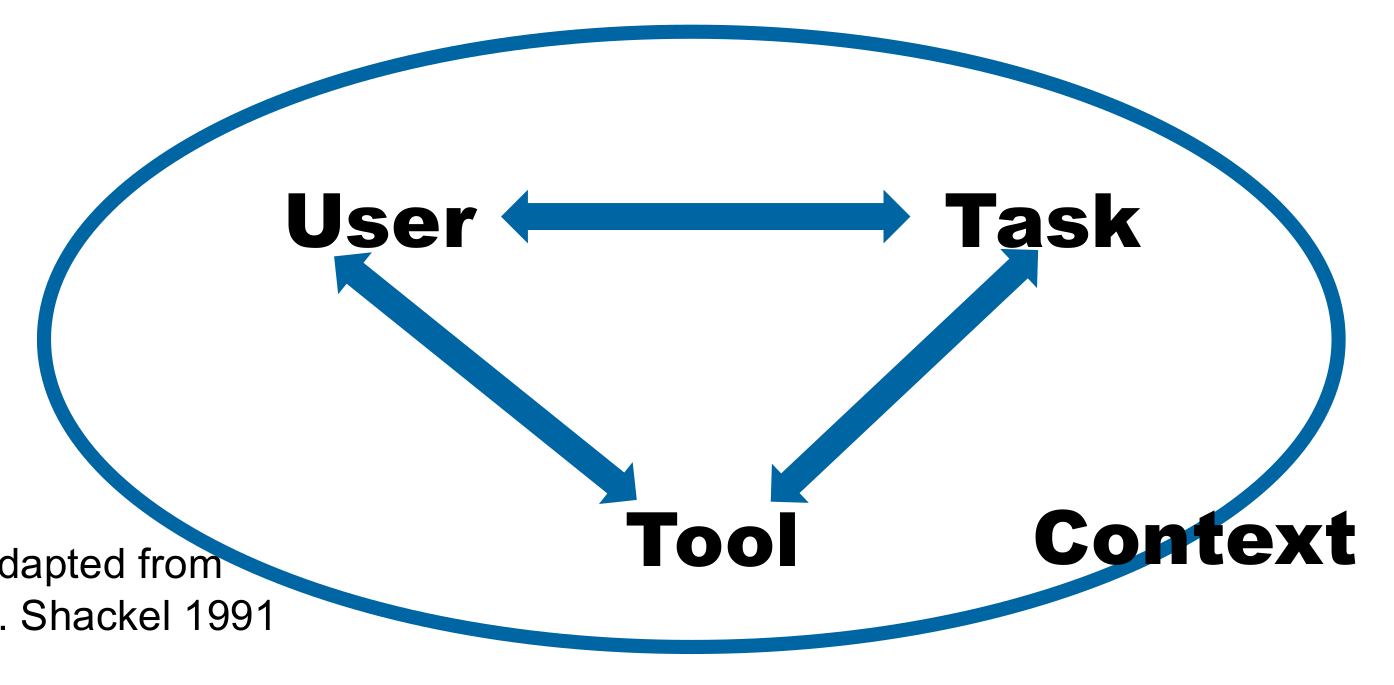
\includegraphics[width=0.15\textwidth]{userToolTask.png}

\subsection{Product Criteria by Stone}
\textbf{Visability:} first step to goal should be clear, \textbf{Affordance:} Control suggests how to use it. Result conforms to expectation generated by control. \textbf{Feedback:} Should be clear what happened or is happening. \textbf{Simplicity:} As simple as possible and task-focused. \textbf{Structure:} Content organized sensibly. \textbf{Consistency:} Similarity for predictability. \textbf{Tolerance:} Prevent errors, help recovery. \textbf{Accessibility:} Usable by all intended users, despite handicap, access device or environmental conditions.

\subsection{User Centered Design Process}
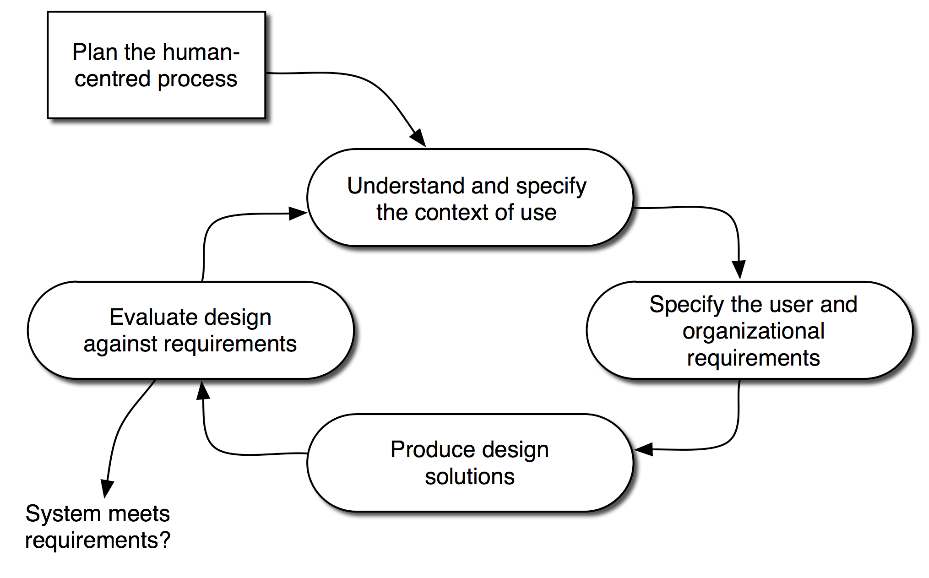
\includegraphics[width=0.15\textwidth]{user_centered_design_process.png}
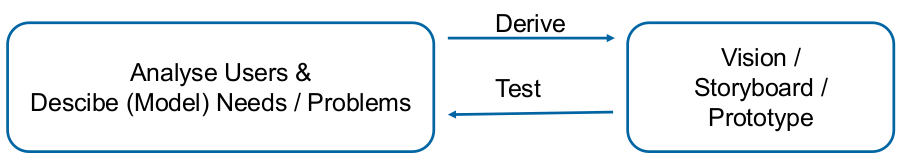
\includegraphics[width=0.15\textwidth]{ucd_process.png}

\subsection{Usability vs User Experience}
\textbf{Usability:} effective, efficient, learnable, error-preventing.
\textbf{User Experience:} value \& meaningful, pleasurable / impressive / memorable, end-toend experience, product \& service experience $\rightarrow$ pre-use: anticipated use, search, unboxing. regular use: first success, usability. post-use: loyality, re-use design, upgrade, replace, recycle. 

\subsection{Garrett's Framework classify Usability}
top(surface) = concrete, bottom = abstract (strategy).
\textbf{surface:} visual design (color, fonts, design). \textbf{skeleton:} interface design, navigation design, information design (layout grid). \textbf{structure:} interaction design, information architecture (navigation, conceptual model). \textbf{scope:} functional specification, content requirements (features).
\textbf{strategy:} user needs, site objectives (target-group, needs, "value", meaning).
UCD Techniques: \textbf{Interviews, contextual inquiry} (strategy, scope | analyse design). \textbf{Scenarios, storyboards} (scope, structure | (analyse) design). \textbf{Wireframes, prototypes \& testing} (structure, skeleton | (design) test).
\\ Benutzerbefragung ist keine User Centered Design $\rightarrow$ People don't know what they want. You have to show it to them first. First rule of usability: Don't listen to users. Observe what they do not what they say. Customer $\rightarrow$ problem expert. Designer $\rightarrow$ solution expert.

\subsection{Scenarios and Personas}
story of the user solving a problem that arises out of logical needs of the situation.
\textbf{Problem-Scenarios} show current (problematic) situations.
\textbf{Future-Scenarios} show users with the same needs and in a similar context as in the problem-scenarios. They illustrate how new tools lead to better outcomes.
Good Scenarios need good personas and good user research. (Garrett: User Segmentation + Selection)
Scenario = Text or Storyboard.
Elements = Problem description(User goal) \& context. User (Persona). Trigger. Steps. Solution (maybe fail).
\textbf{Good Scenarios:} 
should include first success, repeated success (triggered), virality. should have plausible needs, goals, context, trigger, persona. NOT CRUD questions with answers for locations. BUT First use scenario: Peter got a recommendation for the local experts app from a friend .... On the first launch asks permission, he agrees...AND Repeated Success / Triggered Scenario. Peter is in Chur, a place he doesn't know. It is dinner time... remembers the app.
\subsection{Needs}
Apps: I want to share something ("Check In / Status") $\rightarrow$ Social Media, Photo..
I am bored (I want to be entertained / distracted) $\rightarrow$ Games, News..
I want to be productive ( repetitive now, micro tasking) $\rightarrow$ Sort E-Mail, Quick ppt edits.
I want to find something here ( urgent, local) $\rightarrow$ Map, Schedule, Restaurant-Finder (location-based services).

\subsection{Usable in varying use context}
User holing patterns should be respected. Reachability \& touch target size:
Users cognitive limitations should be respected:
Users might be in very noisy (or very quiet) contexts.
Users may be from varying age groups, with varying visual abilities, and in varying lighting situations (contrast, font size, colors).
Users might be in constant mode of distraction (App needs to remind users of its existence, quick results even when users are distracted, interrupted or first time use or long since last use.)
Users in hazardous (resource limited) situations.
Users might show varying levels of involvement.

\subsection{Core Future Scenarios Mobile}
\textbf{Scenario: First success:} 
Why (how, when) was the app installed by the user?
Why is the app used the first time (trigger, motivation to start / to go through all the required steps until success)? 
When is the first time(step) the user gets a recognizable reward/benefit from the use of the app?

\textbf{Scenario: Repeated success:}
Why is the user starting the app again (trigger)?
What are the repeated benefits?
How does the app cater for experts without losing infrequent users?

\textbf{Scenario: Virality}
Why (how) will the user tell others about the app or ge them involved?

\textbf{Phases of app use:} I Attract (visual, desirable) II Delight (information / function, useful and usable) III Retain (repeated use, notifications)
Goal $\rightarrow$ Use power of viral marketing. 26 percent of apps are used only once. Sport apps seems to be used the longest.

\subsection{Mobile vs Desktop}
\textbf{Mobile:} Small screen, input a few characters, slow (or no) network, photograph anything, used anywhere, location aware (mostly).
\textbf{Desktop:} Large screen, type text, fast Internet, photograph user, used when seated, location unaware.) 
$\rightarrow$ Apps should make use of location information: Determine current context: (GPS, WiFi cell, beacons, ambient sound, image reco, sensors(gyro)). Provide info about: (Points of interest, direction, notes (location based notes, leave notes to others), location of friends).

\subsection{Challenge for Apps}
Increase motivation (psychology). Removing Friction (usability) Mountain.
Increase motivation to climb over the mountain or make the mountain smaller.
Apps must provide motivation, ability and trigger:
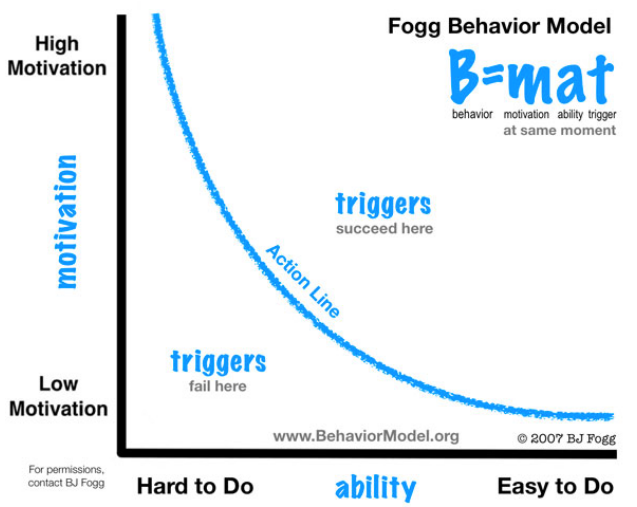
\includegraphics[width=0.15\textwidth]{challenge.png}
Masclow's Hierarchy of Needs: Physiological, Safety, Love/belonging, Esteem, Selfactualization.

\subsection{Techniques of User Centered Design}
ANALYSE - Stakeholder-Analysis, User Interview, Usability Test \& Heuristic Review (current system), Competitive Analysis, Contextual Inquiry / Ethnographic Interview, Persona \& Szenario Modelling, Visioning \& Storyboarding, Card Sorting, Wireframing (Heuristic Review, Hallway Testing), Usability Lab Test - DESIGN
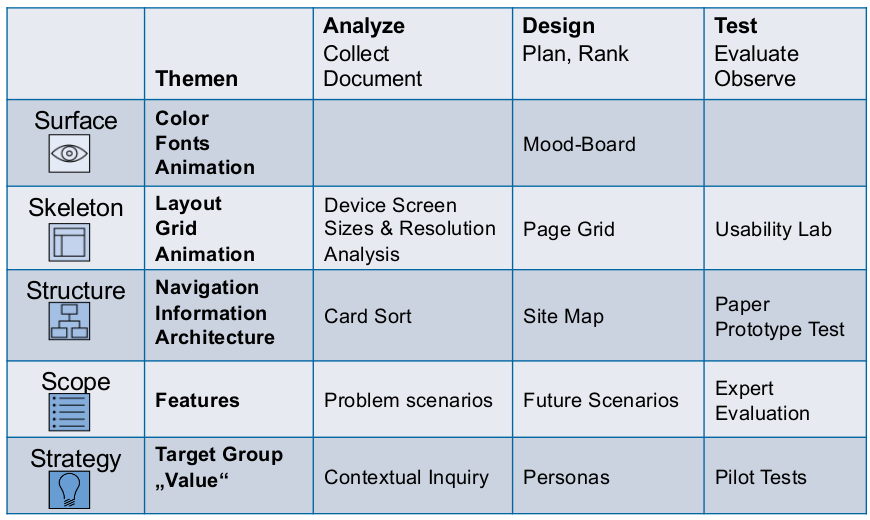
\includegraphics[width=0.15\textwidth]{techniques.png}

\subsection{Mobile Design Process}
Start small (small set of features (1+2), focused target group). Ideation / Concept Development (parallel versions) $\rightarrow$ Identify user needs (hypothesis), validate user needs (Observation, Validate Problem and Future Scenarios). Select one or two concepts for refinement. Refine Concept( Develop "Paper" Mockup for Scenario $\rightarrow$ redesign, validate with walkthrough, test scenarios with mockup $\rightarrow$ redesign) apply platform guidelines $\rightarrow$ retest, Test detail interactions $\rightarrow$ animation). In parallel: remove technical risks. Implement and test scenarios (redesign if necessary).\\
For MSE App: Users, What to observe. How to observe. Hypothesis of needs. Why installed (trigger, motiviation, ability)*. Possible first success scenario *. Possible reuse scenario *. Possible virality scenario *. How to demonstrate validity of scenarios

\subsection{Design Concept}
\textbf{Good Concept-Design:}
Identifies strong situational needs. Identifies a core set of matching scenarios (including Personas)=
Co-evolves tested wireframes, scenarios and needs.
\textbf{Goal must be:}
All features represented as screen flows (sequence of filled wireframes supporting a scenario).
No untested wireframes (No out-of-scenario wireframes). No wireframes without scenario data.
\textbf{Step towards goal:}
1) Create a reasonable empty wireframes collection. Create initial set of scenarios. Walk trhough wireframes. Iterate.
2) Create testable screen flows and test-task description (few at a time).
Validate: Check with Cognitive Walkthrough: do enough pre tests. Plan 3-5 real tests. Iterate

\subsection{Card Sort}
Useful technique to determine navigation hierarchies and naming of menu item.
\textbf{Open Card Sort:} Start with content cards. Let future users create groups and name them (5+ users). 
\textbf{Closed Card Sort:} Start with content cards AND GROUP LABELS. Let future users match content cards to group labels.
IF YOU THINK YOU HAVE TO USE CARD SORT FOR APPS THEN IT POSSIBLY HAS TOO MANY FEATURES.

\subsection{Screen Map}
Lists all screens of an app, groupings and major navigation links.
The screen map for horizontal tablets might differ from the one vertical tablets or for small screens.
Horizontal tablet layouts often combine multiple views.
They show descendant and lateral navigation (also maybe back and up). Show List, Grid, Carousel, simple buttons, dashboard, tabs, swipe etc.
\textbf{Abstract Screen Map} Home, Photo List, Photo View. Story View etc.
\textbf{Wireframe Screen Map} Show the screens and what happens if menu button is pressed etc.

\subsection{Prototyping, tools and usability testing}
Using just paper, can be faster and more efficient for testing. Tools can be used to make the same electronic for Interaction, Animation, Gestures, Design, Demoing, Documentation, Responsive Design (Marvel for example). \textbf{Usability testing challenges:} Defining good scenarios with plausible needs, goals, context, trigger. persona (user can log in is bad). Creating inexpensive and quickly the needed screen flows for testing (not collection of empty wireframes). Creating matching task descriptions that communicate needs... (not log in as user: test-user, pw 123). Inviting the right test persons (beware of friends and family). Making test persons understand that the system/concept is tested (pre- and post- questionnaire). Make test persons think aloud (let them read the description than they should continue with talking. Only controlled help).

\subsection{Co-Developing Screen Flows \& Test Tasks}
Scenarios are the basics for creating screen flows and description of the test tasks. Test tasks specify: user context, need, goal and trigger. Do not specify: specific terms that should be used, specific steps that should be taken. Example triggered task: see Scenarios and Personas. Screen flows include the data that would be entered for an optimal task performance.

\subsection{Testing Mistakes}
1 Recruiting unsuitable participants. 2 Not testing early and often. 3 Following a test plan too rigid. 4 Not rehearsing the setup. 5 Using a one-way mirror. 6 Not meeting participants in reception. 7 Asking leading questions. 8 Undertaking two roles in testing session. 9 Not considering external influences.
\textbf{Things that can go wrong}
1 Users don't show up. 2 Facilitators gets sick. 3 Internet goes down. 4 Awkward moments. 5 Distractions. 6 Users are quiet. 7 Software stops working. 8 Takes too long. 9 Forget to record the time. 10 Video didn't record.

\subsection{Designing App Skeleton (Pages + Grid)}
Difficult to know what screen size user will interact with the app. Goal should be achievable on all devices and orientations. Knowledge about orientation and device can help to optimize. Tablets are more used at home and older people. Holding patterns should be used to optimize visibility.
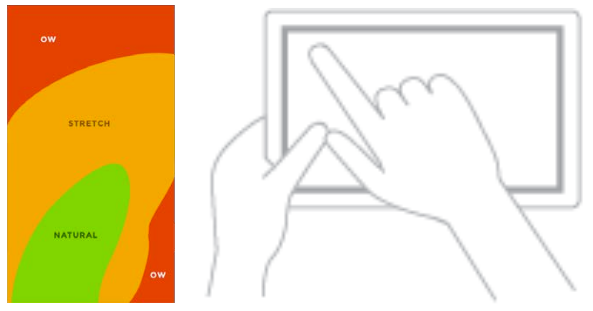
\includegraphics[width=0.15\textwidth]{holding.png}
Touch targets should be at least $1cm^2$. Best is 0.9cm + 0.2cm padding. (more space needed inf used in stressful situations)

\subsection{Mobile Design Pattern}
Empty Datasets: You haven't liked any photos yet.
Spingboard: Like like tic tac toe.
List Menu, Tab Menu, Gallery.
Primary Navigation (Transient) $\rightarrow$ Side Drawer, Popup Menu.
Secondary Navigation $\rightarrow$ Page swiping (hor or vert).
Tips:
Make primary actions obvious: High-contrast button affordance.
Segmented Control instead of Toggle Menu.
ZIP instead City state zip.
Inline validation: did you mean gmail.com
Use Switch Slider Segmented Controls.
Mobile first, don't port Desktop UI to mobile.

\subsection{Design in Mind}
Error message close to action. Keep in mind that 9 per cent of men have color vision deficiency.
\textbf{Mistakes:} Too many steps to first success (create profile, tutorial). Touch areas too small. Non standard controls. Android users designing for iOS or vice versa. Web designers designing for mobile. Corporate Design and marketing knows it better...

\subsection{Android Guideline}
Has a back button and app stack (Back != up).
Put back button in app is bad (if necessary provide up button), same with exit button.
\textbf{Antipatterns:} Splash screen (better image placeholders), tutorial screen (better explain in time, context), Confirmation window (better provide undo), Menu button (outdated), Hiding status bar, sipe overlay quick actions, using non-android design. Don't mix actions and navigation in a single bar.

\subsection{IOS Platform Guideline}
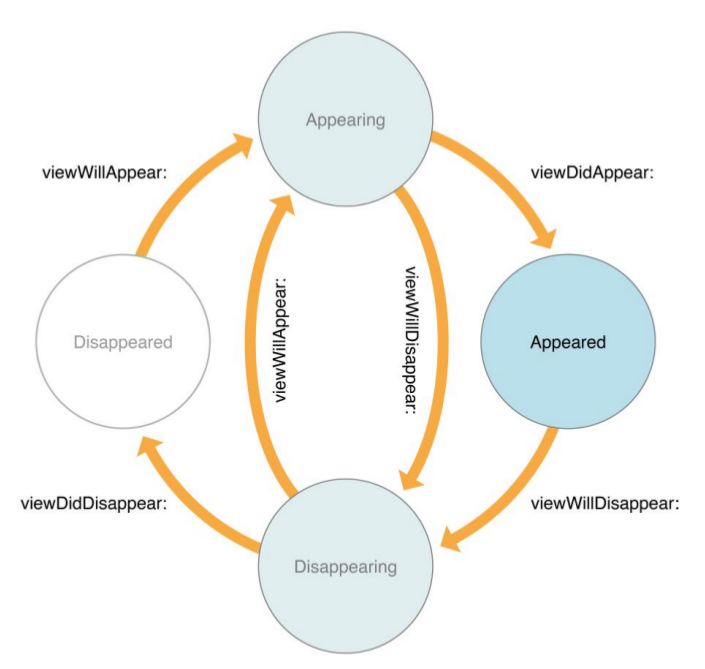
\includegraphics[width=0.15\textwidth]{ioslife.png}
The iOS HIG (Human Interface Guideline) is like material design but for ios (Overview, Interactions, Features, Visual Design, Graphics, UI Bars, UI Views, UI Controls, Extensions, Technologies, Resources, Related Guidelines). Consider putting a segmented control in a navigation bar at the top level of an app. Helps to flatten the information hierarchy, making it easier to find things. Be sure to choose accurate back button titles. The Floating Action Button is not that good, better right side of navigation bar or tool bar. iOS needs close buttons! iOS design: everything clickable no side menus, better no side menus in iOS. Google has side menu integrated (older than 40 not used to click on hamburger icon to get to menu). Tab-bar new at the bottom for both system.
Modern take swift: Statically, strongly typed. Compiler can often infer types (type annotation can often be omitted). Compiles to native code. No main, semicolons required. print() is defined in the Standard library (implicitly imported). Only file which can contain top level code is main.swift (else top level declarations). Goal: safer, more flexible more fun more than Objective C (interoperability).Integer overflow traps. + Better chance to find overflow bugs. + Well defined behavior. - Requires run-time checks. Has types Int, Float, Double, String, Bool, Array<T> or [T], Set<T>, Dictionary<K,V> or [K:V]. All have value semantics. Some use coopy on write in order to be efficient. Are nominal types: can be extended (initializer (ctor) methods etc.) 
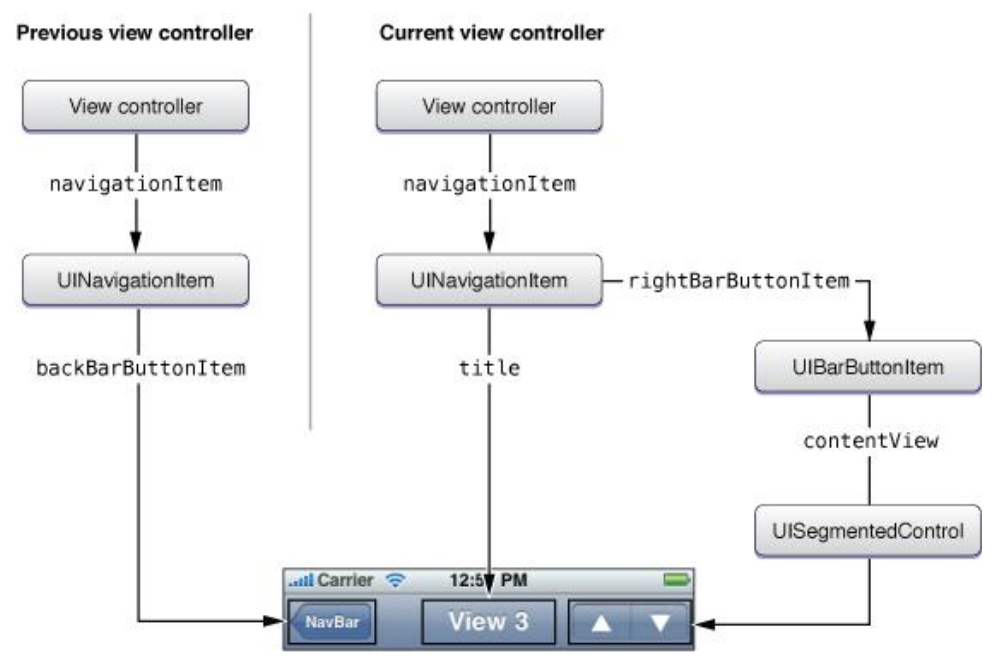
\includegraphics[width=0.15\textwidth]{navigationbar.png}
ViewControllers=each controls a view and its subviews. There are methods/hooks for when a view controllers view i sloaded, appears, disappears (ViewController Lifecycle). viewDidLoad() main and subviews are loaded from the interface builder, bus size and position may not be set yet. Good method to change background color, add additional subvies, change text labels etc.

\subsection{Material Design}
\textbf{Principles:} Material is the metaphor: Elevation of materials, what is above which element, how height. Bold, graphic, intentional: typography, grids, color, scale, space, create hierarchy, meaning, focus. Motion provides meaning: focus attention, giving feedback.
\textbf{Components:} Bottom Navigation. 
\textbf{Patterns:} Empty States: image = neutral, purpose and potential like icon, positive tone, consistent with brand, should not look like it's an action. Permissions: simple, transparent and understandable. Should clarify why permission is needed. Runtime permissions = at the moment user needs to perform action. Denied permissions should provide feedback and options. Types of permissions: educate before asking, ask up front, ask in context, educate in context, provide an immediate benefit, only ask for relevant permissions. Scrolling: Use flexible space to accommodate images in the app bar with the desired aspect ratio. 

\subsection{Agile SW Development}
DESIGN (create mockups) $\rightarrow$ DEVELOP $\rightarrow$ COMPILE $\rightarrow$ TEST $\rightarrow$ REFACTOR \\
COMPILE DISTRIBUTION VERSION $\rightarrow$ TEST $\rightarrow$ RELEASE/PUBLISH \\

\subsection{Costs}
40k for a kart, 100k for a Skoda, 500k for a BMW, 1mio+ for a Rolls Royce. Switzerland iPhone Country (2/3 : 1/3) but worldwide android 80-90. \textbf{When go native:} If security is very important (SDKs NDK), Performance or resource optimization (battery, memory), Use newest technologies (APIs, wearables etc), When only one platform must be supported. Pixel perfect UIs. \textbf{When go cross:} Low budget, only basic requirements for UI, Web programming skills available but no native skills, prototyping or proof of concepts, Game engines, 3D visualization (unity). Mostly it's not as much faster to implement and not much less cost as expected. 60 per cent is not yet using swift.

\subsection{Swift}
Swift is statically typed (types known at compile time), strongly typed (there aren't a lot of implicit type coercions (pass int instead of double needs cast)), compiler can often infer types (type annotations can be omitted), uses automatic reference counting (ARC) for memory management. Compiles to native code (doesnt run in virtual machine), may rely on Objective-C runtime (not available on linux). No main() required. print() defined in standard library (implicitly imported). Only main.swift can contain top-level code (all others only top level declarations). Goals = safer, more flexible more fun than Objective C. Each significant change is described in a proposal (Markdown). idea mailing list - write proposal - request review - core team member who accept pull request becomes review manager - number assigned - anyone can review - core team decides if accepted rejected or deferred.

\subsection{Numeric Types}
Some of the types use copy-on write in order to be efficient. They all have value semantics. Are nominal types (can be extended).
var x = 2, x += 2 Int,
let y = 4.5 Double
,let z: Float = 4.5 Float,
let (d1,d2) = (2,4.5)
func f(\_x: Double) {}
,f(x) cant convert Int to Double
,f(4) works integer literal

\subsection{Strings}
Are unicode-compilant, value semantics, different views for various unicode representations.
var str = "Hello", str += " x!" (x = emoji),
for c in str.characters {print(c)} = human readable characters,
str.characters.count = 8,
str.utf8.count = 11,
str.utf16.count = 9,
str.uppercased(),
str.lowercased()

\subsection{Arrays}
have to be same type, value semantics, empty array [], [Int] = Array<Int>\\
let ints1 = [1, 2, 3, 4, 5] //Array<Int>
, var ints2 = ints1 // mutable copy
, ints2.append(6) // here copy
, print(ints1)
, let strs = Array(repeating: "Hi", count: 10)
, for s in strs { ... }
, for (i, s) in strs.enumerated() { ... }
, ints2[0...<3] = [0, 0]
, ints2[0...4] = []
%\begin{lstlisting}
%let ints1 = [1, 2, 3, 4, 5] //Array<Int>
%var ints2 = ints1 // mutable copy
%ints2.append(6) // here copy
%print(ints1)
%let strs = Array(repeating: "Hi", count: 10)
%for s in strs { ... }
%for (i, s) in strs.enumerated() { ... }
%ints2[0...<3] = [0, 0]
%ints2[0...4] = []
%\end{lstlisting}

\subsection{Sets}
Elements needs to conform Hashable protocol. Value semantics.\\
, var letters: Set<Character> = []
, for c in "it is a test".characters {
	letters.insert(c) }
, if letters.contains(" ") { // compiler knows its char not str
	print(letters.count) }
%\begin{lstlisting}
%var letters: Set<Character> = []
%for c in "it is a test".characters {
%   letters.insert(c) }
%if letters.contains(" ") { // compiler knows its char not str
%   print(letters.count) }
%\end{lstlisting}

\subsection{Dictionaries}
keys need to conform to Hashable protocol. value semantics, empty dictionary [:]
[TypeK:TypeV] = Dictionary<TypeK, TypeV> \\
, let population = ["Switzerland" : 8\_000\_000,
, "Germany" : 80\_000\_000]
, for (country, count) in population {
	print("\\(country): \\(count) people") }
, print(population["Germany"])
, print(population["Italy"]) // nil
, population["France"] = 66\_000\_000 //new
, for k in population.keys { }
, for v in population.values { }
%\begin{lstlisting}
%let population = ["Switzerland" : 8_000_000,
%                       "Germany" : 80_000_000]
%for (country, count) in population {
%   print("\(country): \(count) people") }
%print(population["Germany"])
%print(population["Italy"]) // nil
%population["France"] = 66_000_000 //new
%for k in population.keys { }
%for v in population.values { }
%\end{lstlisting}

\subsection{Tuples}
Tuples, function types, any, anyobjects cant be extended !
multiple values into single compound value, can have different types, no single-element tuples Type(Int) = type int. Expression ("hello") = type String not (String). Empty tuple () is a valid type. Has a single value, same as Void \\
let john = (33, "John") // (Int, String)
, print("\\(john,1) is \\(john.0).")
, let dora1 = (age: 26, name: "Dora1")
, var dora2 = dora1
, dora2.name = "Dora2"
, dora2.age += 1
, print(\\(dora2.name) is \\(dora2.age))
%\begin{lstlisting}
%let john = (33, "John") // (Int, String)
%print("\(john,1) is \(john.0).")
%let dora1 = (age: 26, name: "Dora1")
%var dora2 = dora1
%dora2.name = "Dora2"
%dora2.age += 1
%print(\(dora2.name) is \(dora2.age))
%\end{lstlisting}

\subsection{Function Types ** buggy}
func f1() {}  // (()) -> () **
, func f2(\_x: Int) -> Int { return x } // (Int) -> Int
, func f3(\_x: Int, \_y: Int) {} // ((Int, Int)) -> () **
, func f4(\_x: (Int, Int)) {} // ((Int, Int)) -> Int
%\begin{lstlisting}
%func f1() {}  // (()) -> () **
%func f2(_x: Int) -> Int { return x } // (Int) -> Int
%func f3(_x: Int, _y: Int) {} // ((Int, Int)) -> () **
%func f4(_x: (Int, Int)) {} // ((Int, Int)) -> Int
%\end{lstlisting}


\subsection{Any vs AnyObject}
any: existential type without requirements, build into compiler, all types are implicit subtypes of it \\
func f(\_x: Any) {}
, class C {}
, let c = C()
, f(c)
, f(2)
, f((0.5, "test"))
, f([true, false, true])
, f(f)
%\begin{lstlisting}
%func f(_x: Any) {}
%class C {}
%let c = C()
%f(c)
%f(2)
%f((0.5, "test"))
%f([true, false, true])
%f(f)
%\end{lstlisting}
They all work. If AnyObject instead of Any it has to be a class. Only f(c) works. (class requirement)
Never: uninhabited type in stl (doesnt have any value) public enum Never{}, means that function can not return, examples fatalError() exit(), they can be used in else-clause of guard statement.

\subsection{Frameworks}
Cocoa Touch = \textbf{UIKit}, Push Notification, MapKit, MessagUI, AddressBook UI, EventKit UI, GameKit
Media Layer = Core Animation, Core Image, Core Graphics , OpenAL, OpenGL.., Core Text, Core Audio, Image /O
Core Services = Core Data, \textbf{Foundation}, Core Foundation, SQLite, Address Book, XML Support, Store Kit, Core Location, System Configuration, Core Media, CFNetwork.
Core OS = System(Kernel, UNIX Interfaces), Security

\subsection{Structure of an App}
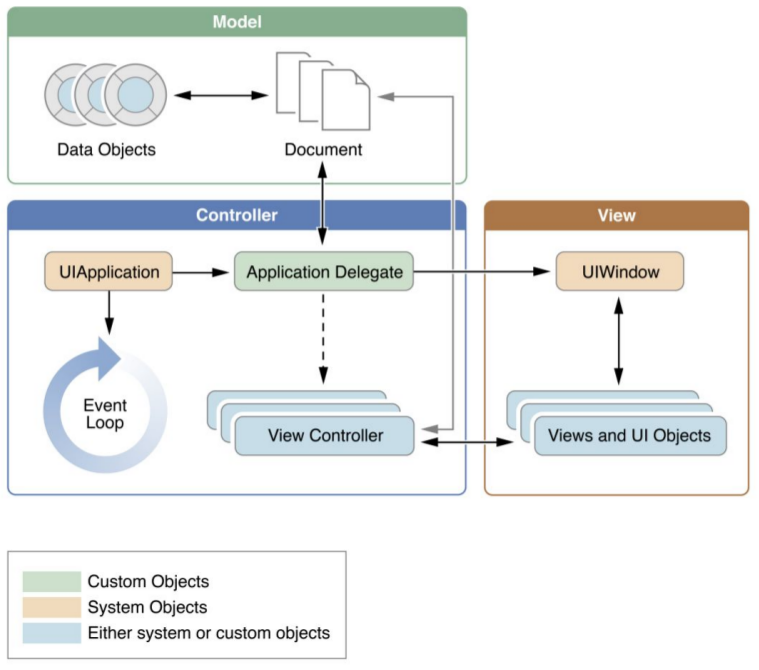
\includegraphics[width=0.15\textwidth]{appstructure.png}

\subsection{Networking with URLSession}
URLSession + related classed provide a complete networking API. Part of the Foundation framework. Also available on linux.
URLSessionConfiguration $\leftarrow$ URLSession $\rightarrow$ (creates) URLSessionTask $\leftarrow$ URLSessionDataTask or URLSessionDownloadTask or URLSessionUploadTask. URLSessionTask = A task represents a specific download / upload. Tasks are created using URLSession's factory methods. All tasks start in a suspended state. Call resume() to start the task. Completion handler is executed on background thread.
